\section{Tool Support}
\label{sec:tool}
\begin{figure}
    \centering
    \begin{subfigure}{.365\columnwidth}
    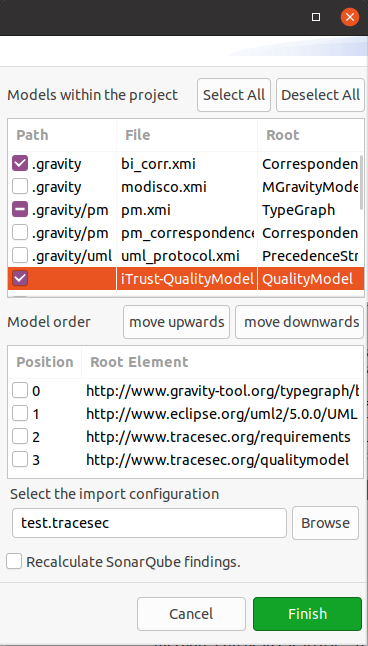
\includegraphics[width=\columnwidth]{figures/tracesec-impl-selection.png}
    \caption{Selection Wizard}
    \label{fig:wizard}
    \end{subfigure}
    \begin{subfigure}{.61\columnwidth}
    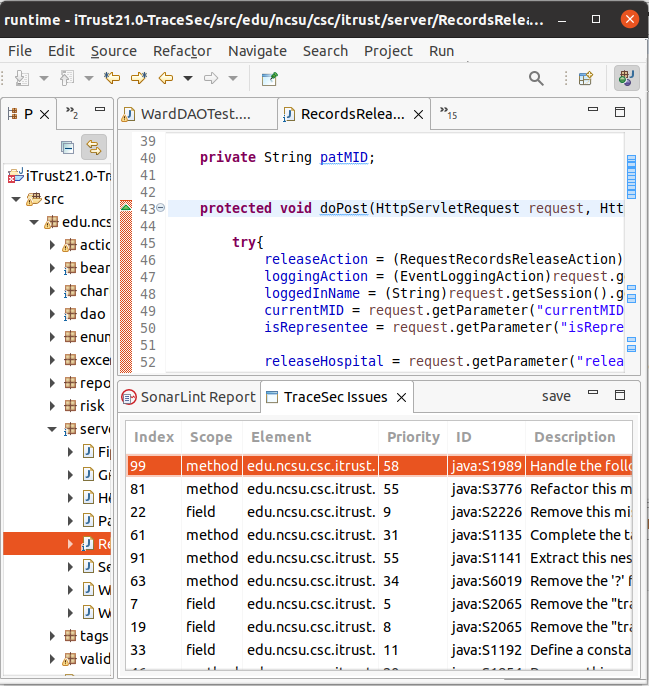
\includegraphics[width=\columnwidth]{figures/tracesec-impl-results.png}
    \caption{Result Presentation}
    \label{fig:results}
    \end{subfigure}
    \caption{Screenshots of the Tool Support}
    \label{fig:impl}
\end{figure}

We implemented \appr{} in Java with an Eclipse\,\cite{eclipse} plugin as a front-end for integration with the Eclipse IDE.
The tool introduces a wizard for calculating priorities for a Java project.
\autoref{fig:wizard} shows the UI of the wizard for selecting the models to be considered in the prioritization.
In the upper half, the user selects the quality model, the program model, models containing trace links, and other models to be considered, such as requirements or UML models.
The tool uses the EMF for models.
In the lower half, the user arranges the selected models to define the order of the artifacts from which the tool calculates the distance between model elements needed to compute the flow in the flow network. In addition, the user specifies a configuration file that declares project specific capacities and ignores certain types of relationships using the DSL we provide, as shown in an example in~\autoref{dsl}.
The SonarQube issues are calculated (if not already present) and added as annotations to the program model.

The prioritization view (bottom of \autoref{fig:results}) shows the issue findings in a list view, giving details about their id, scope (\emph{class}, \emph{method}, or \emph{field}), location, issue description, and the priority as automatically calculated by \appr.
The table view allows navigating to each issue in the code on click.
%

To specify the artifact import specification using the DSL introduced in \autoref{sec:dsl}, we implemented this DSL using the language engineering toolkit  Xtext\,\cite{xtext}.
Given a grammar such as the one shown in \autoref{lst:grammar}, Xtext allows the generation of parsers and runtime editing support integrated into IDEs\,\cite{BPA+2022}.
Internally, Xtext is based on EMF for providing access to the parsed DSL instances, which allows explicitly referencing types from EMF-based metamodels, i.e, EMF-based implementations of the UML\,\cite{Gerard2007}, BPMN\,\cite{EclipseBPMN}, data flow diagrams (DFDs)\,\cite{Tuma2019}, or Palladio\,\cite{reussner2011palladio}.
In this way, the DSL allows immediate interaction with EMF models, including editing support such as auto-completion, even for elements specified in imported EMF metamodels, syntax highlighting, and validation.
Since Xtext supports the Language Server Protocol (LSP)\,\cite{lsp}, this editing support is not limited to the Eclipse IDE, but can serve any IDE that supports the LSP\,\cite{BPA+2022}.
We provide instances of this DSL (cf. \autoref{dsl}) to support the quality model used by \appr{}, requirements models based on a metamodel we created to capture the requirements of iTrust that is oriented on the requirements relation model of Großer et al.\,\cite{Grosser2022RDR}, UML models\,\cite{uml}, and the GRaViTY program model\,\cite{gravity,Peldszus2022}.
We also provide the EMF metamodels for the quality model and the requirements model.
While we provide automated tool support for linking issues detected by SonarQube to elements of the GRaViTY program model, as all models except for the quality model, this model can be replaced by any other model that captures the source code of the system.
Still, we recommend the GRaViTY model since it is language independent, provides an abstraction that minimizes the size of the flow model, and unlike many source code representations, such as abstract syntax trees, it contains explicit references for representing accesses to members instead of just names of methods or variables.

In addition to the Eclipse plugin, the metamodels for the quality and requirements models, and the DSL, we provide standalone executables for automating the tasks described in our evaluation in \autoref{sec:eval}.
The Eclipse-based tooling and our evaluation-related tooling are provided in our replication package\,\cite{replication}.

\section{Evaluation and Discussion}
\label{sec:eval}

We evaluate \appr{} with respect to four objectives:

\begin{enumerate}[label=\textbf{O\arabic*:}, ref=O\arabic*]
    \item \textbf{Effectiveness:}
   		How effective is \appr{} in prioritizing issues?\label{o1}
    \item \textbf{Adjustability:}
    	How well can \appr{} be adjusted to project priorities?\label{o2}
    \item \textbf{Robustness:}
    	How much do trace links influence the issue prioritization?\label{o4}
    \item \textbf{Performance:}
   		How does \appr{} scale for input data of varying sizes?\label{o3}
\end{enumerate}

First, we evaluate how effective \appr{} is in prioritizing SonarQube issues on two real-world Java projects---iTrust and the server component of the German Covid-19 warning app~(CWA)\,\cite{cwa-server}---and compare the automated prioritization with \appr\ with a manual one and severities provided by SonarQube.
While \appr{} should work with any static analyzer, we selected SonarQube due to its popularity and availability of rule severities for comparison.
\edit{%
    While SonarQube offers rules explicitly labeled as security rules, we decided to consider all rules for two reasons.
    First, many rules not labeled as ``security'' rules can be still relevant for a system's security. For example, the rule that detects buffer overflows---the cause of many security issues such as the injection of arbitrary code by an attacker\,\cite{Cowan2000}---in C programs is not labeled as a ``security'' rule but to address ``reliability'' issues.
    Second, in practice all rules are executed and there is the danger that the many findings concerning qualities such as ``maintainability'' hide the detected vulnerabilities.
}
In the second part of our evaluation, we investigate how well the prioritization can be adjusted to project-specific quality requirements by investigating the impact of the quality model's priorities on the prioritization.
Afterward, we analyze how robust the approach behaves with respect to incomplete or incorrect trace links.
Finally, we investigate how well the construction approach scales for input data corresponding with software projects of different sizes.
Our implementation and all evaluation data can be found in our replication package\,\cite{replication}.

%For the CWA, identified threats and considered security properties threatened are documented and were easily translated into a quality model.

\subsection{Evaluation Use Cases}
This section introduces the software applications used as evaluation use cases, including the artifacts that are used as input for the evaluation. We publicly provide all artifacts built for the evaluation use cases\,\cite{replication}.

\subsubsection{iTrust}
% What was mentioned, what is not mentioned (yet)
% QM: source, descr, numbers
% Req: source, descr, numbers
% Arc: source, descr, numbers
% Code: source, !numbers (loc?)
% QM -> Req: source, descr
% Req -> Arc: source, descr, numbers
% Arc -> Code: source, descr, numbers

The iTrust\,\cite{heckman2018} electronics health records system is a software application for managing patient data, appointments and medical records in healthcare organizations. It handles sensitive personal medical data, which implies security as a relevant quality property.
The system is implemented using Java Server Pages and 77,501 logical lines of Java source code in the version 21 used in our evaluation.
Its source code and documentation are publicly available.\footnote{\url{https://github.com/ncsu-csc326/iTrust}}
The iTrust use case is used as a running example in \autoref{DevArt}.

The documentation of iTrust\,\cite{iTrustWiki} lists 79 use cases as requirements, of which 36 requirements are implemented in version 21.
The structure of these requirements was shown in the running example used above (see \autoref{fig:uc26}).
From these textual requirements documents, structured by DokuWiki\,\cite{dokuwiki} page structure elements such as headings and hyperlinks, we derived a requirements model\,\cite{Grosser2022RDR} by parsing the requirements documents and automatically mapping the parsed content to the requirements model structure.

We created a quality model for iTrust based on its documentation. The quality model includes 11 qualities, with \emph{Authentication}, \emph{Logging}, \emph{Integrity}, and \emph{Secrecy} as the highest-level qualities. In the best case, the quality models used in this evaluation would already have been created as an additional artifact of a threat analysis, e.g., following STRIDE\,\cite{STRIDE}, which is already part of the software development process in many security-critical domains.
However, to perform such a threat analysis and create a quality model for iTrust, as shown in this work, after the fact by screening all requirements, we needed two working days. Still, from a security engineering perspective, such artifacts should be developed up front, and the fact that our approach uses them is an added benefit.

We extracted the structure of iTrust in the form of UML class diagrams through static code analysis\,\cite{Peldszus2022,gravity}. It comprises classes and interfaces of 936 Java source files, their relations, attributes and operations. Correspondences between structural elements and the requirements were documented by the iTrust developers in the iTrust wiki.
We transformed these traces into 184 correspondences that are captured in a correspondence model\,\cite{schurr1994specification} that persists these correspondences and allows to trace between the UML model and code.


\subsubsection{CWA Server}
% What was mentioned, what is not mentioned (yet)
% QM: source, descr
% Req: non-existence
% Arc: source, !descr, numbers
% Code: source, !numbers (loc?)
% QM -> Arc:  source
% Arc -> Code: desc.

The Corona WarnApp (CWA)\footnote{\url{https://www.coronawarn.app}} is an open source software system for warning citizens regarding a potential risk for a COVID infection, and vaccine certification management.
The CWA warned users in Germany until April 2023 with an estimated user base of 27 million users.\footnote{\url{https://www.coronawarn.app/en/science/2022-03-03-science-blog-5/\#4-estimations-of-the-active-users}, accessed 2023-06-14} Since May 2023 it serves as certification management system.
The application comprises apps for iOS and Android on the client side and a server connected to the client apps as well as other servers operated by the German government.
This evaluation use case only considers the server side, which is implemented as a Java application with 17,799 lines of code.
Since the server specifically handles encryption keys for user notifications, security is an important issue.

Unlike iTrust, the CWA server evaluation use case did not use a requirements model because no explicit server-side requirements were publicly available at the time of the evaluation.
However, the architecture of the CWA application is publicly documented\footnote{\url{https://github.com/corona-warn-app/cwa-documentation/blob/main/solution_architecture.md}, accessed 2023-06-14} with box-and-line diagrams for structure, UML sequence diagrams for behavior, and informal text. We replicated the architecture using the UML 2 profile for EMF based on the architecture documentation and source code analysis to create trace links to the implementation. The server consists of 17 components and 6 interfaces and their interrelationships.
The components are implemented in code as Maven projects.
With respect to user-defined security prioritization, as captured in the quality model used in \appr{}, the risk assessment of the CWA server is publicly documented.
The developers have built a threat model in an official Privacy Impact Assessment (following the European Union's General Data Protection Regulation\,\cite{GDPR2016}) that identifies security risks, threats, and associated control measures\,\cite{CWA.DSFA.v1.20, CWA.DSFA.A8}.
The document contains assessments of each identified security risk against nine general threat categories (Data Minimization, Confidentiality, Integrity, Availability, Authenticity, Resilience, Controllability, Transparency, and Appropriateness) using a numerical value that represents the impact if the risk were to occur.
We filtered these for security risks related to the CWA server and transformed them into a formal quality model.
The quality model contains the identified threats as nodes on its first layer and the risks on its second layer, where the risks are linked to the threats based on their severity in the risk assessment document.
We did not add any additional information in this process.
We then mapped the risk nodes to the architectural elements based on which parts of the software systems are mentioned in the textual descriptions of the risks.
Since only a PDF containing tables was available, this transformation was performed manually in less than 30 minutes.
If the source format had been available, presumably in the form of spreadsheets, this step could have been automated without changing the security experts' workflow.

\subsection{Effectiveness}
To evaluate the effectiveness of \appr{} (\ref{o1}), we compare issues prioritized automatically by \appr{} and the severities provided by SonarQube with a manual prioritization.

Although other prioritization techniques exist (see \autoref{sec:rw}), most related techniques mainly consider different quality aspects, such as technical depth in general, or focus on single narrow types of vulnerabilities and would therefore make a bad comparison, or focus on identifying false positives, which is a different kind of problem.
Furthermore, the necessary tools are either not publicly available or the prioritization is mainly based on manual effort.
	However, SonarQube's rule priorities are one of the most important factors for prioritization in practice, as they are prominently displayed through interfaces to SonarQube, such as SonarCloud\,\cite{sonarcloud}.

\begin{figure}
	\centering
	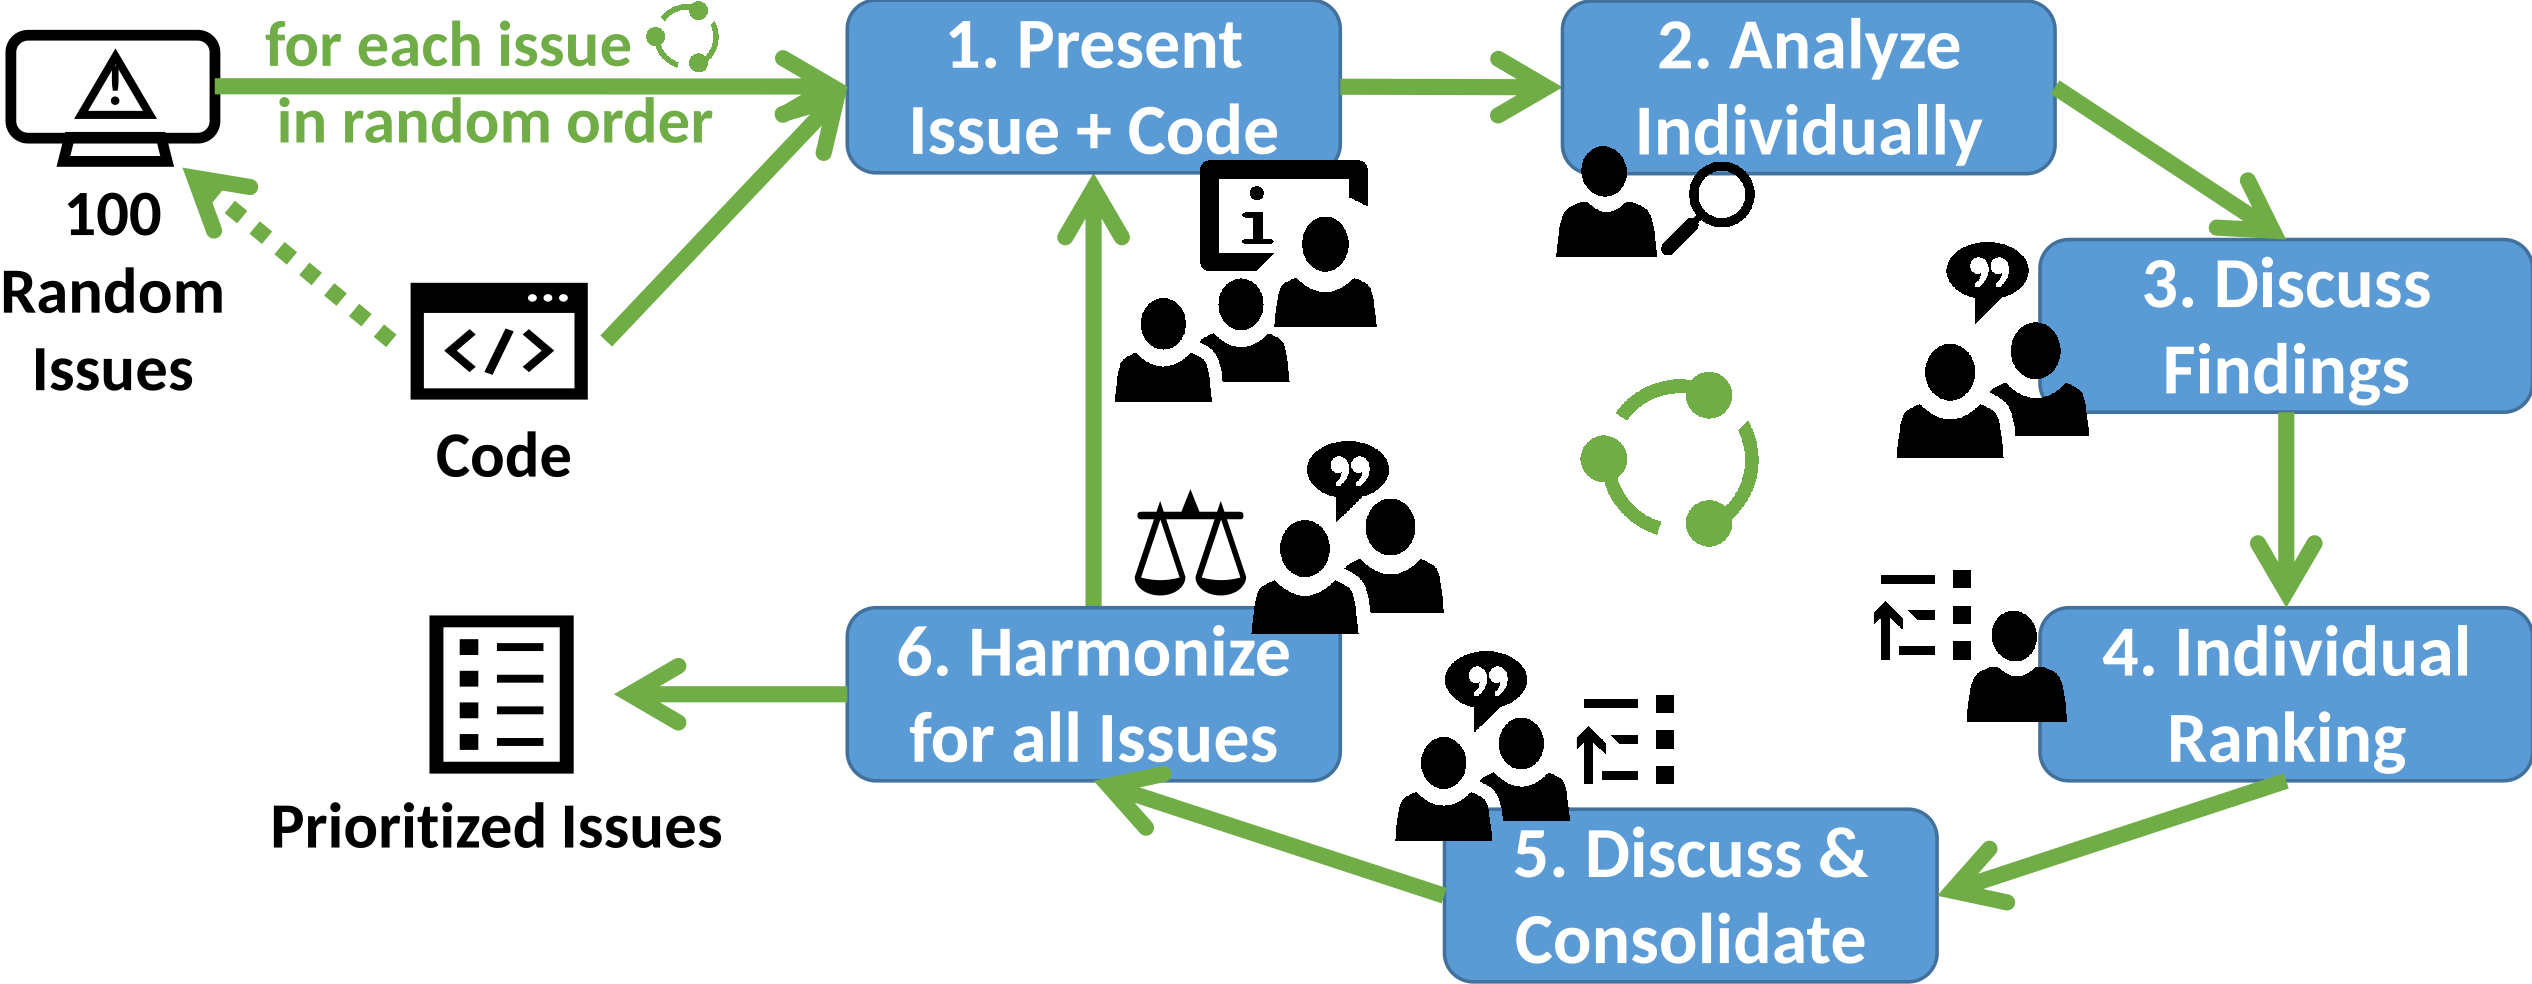
\includegraphics[width=.6\columnwidth]{figures/ManualPrio-KG.png}%width=0.8\textwidth
	\caption{Manual Issue Prioritization Workflow}
	\label{fig:ManualPrio}
\end{figure}

\subsubsection{Setup}
%We extracted randomly a set of 100 issues from the 6,284 ones calculated with SonarCube for iTrust and prioritized these manually before the results of the automated prioritization of the maximum flow analysis were known.
We randomly extracted two sets of 100 SonarQube issues each from iTrust's 6,284 issues and 159 issues calculated for the CWA. %the 159 for CWA.
We prioritized these manually before the results by applying \appr{} were known.
The rating was determined in group discussion sessions with four of the authors as illustrated in \autoref{fig:ManualPrio}.
Each issue was categorized from 1~(low) to 10~(high) %low to high %between 1 and 10
concerning its urgency to fix based on its security impact.
For that, its type and code location are taken into account in steps 2-5 in \autoref{fig:ManualPrio}:
\begin{enumerate}[label=\alph*), ref=\alph*)]
    \item What is the purpose of the code at the given location?
    \item What is the relevance for the project?
    \begin{enumerate}[label=\roman*), ref=\roman*)]
        \item Is it productive or test code?
        \item Is it a main functionality related to a requirement?
        \item What is the security relevance of the handled data?
        \item How accessible is the location from outside the system?
        \item How exploitable is the source code at the given location?
    \end{enumerate}
    \item Which security qualities (from the Quality Model) are addressed by the issue?
\end{enumerate}

\begin{figure}
    \centering
    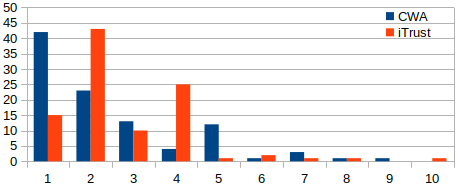
\includegraphics[width=.6\columnwidth]{figures/manual-rankings}
    \caption{Distribution of the manual issue priority categorizations for the two case studies.}
    \label{fig:manual-ranks}
\end{figure}

After a short discussion, full agreement was reached among all raters for each score.
In total, the rating took $\approx$120~min per project.
\autoref{fig:manual-ranks} shows how the 100 issues were ranked for the two case studies.
The majority of issues, 65 for CWA and 58 for iTrust, were rated with a priority of 2 or less. Only 6 issues for CWA and 5 for iTrust have a priority of 5 or higher, representing the group of most important issues for the projects.

%Trace dependencies are used by the tool to make up for the intuition about the code that the developer has, but the tool does not have.

The automated \appr\ approach does not categorize the issues from 1 to 10 but assigns different values, based on the maximum flow that reaches the issue.
SonarQube labels issues with five different severities ranging from \textit{Info} to \textit{Blocker} to which we assigned values from 0 to 4.
However, as the goal is to prioritize the findings, the absolute numbers are not relevant.
What we are interested in is the ordering. We compare the three rankings of the same 100 issues.

\subsubsection{Results}
%
In a first comparisan, to study the general alignment of the prioritizations, we compared the prioritizations using the Spearman rank correlation coefficient\,\cite{10.2307/1412159}.
\autoref{tab:correlations} shows the %calculated
R-values and the significance level at which our results are significant.
These R-values indicate that all correlations are significant at a significance level of 0.01\,\cite{Whitlock2008ABD}.
The rankings calculated using \appr{} correlate much stronger with the manual rankings than SonarQube's severities.
In line with our basic assumption,  only very few issues ($\approx$4\%) are considered to be highly important for iTrust, in the manual and our approach's ranking. In particular, only one is rated 10 manually---while there are very many critical issues according to SonarQube's severities---one fourth of all issues.
We made the same observation for the CWA.
Generally, \appr{} and the manual rankings agree upon issues being low, medium, or highly relevant.
E.g., for iTrust, the 40 lowest rated issues are the same in both orderings and besides one outlier all issues manually rated as important also got a high priority by \appr.
Yet, within these clusters of similar weights, the issues are shuffled. %negatively impacting the correlation.
This is not surprising, as the manual prioritization and SonarQube's severities are less fine-grained than \appr{} and an absolute order is hard to define.
These permutations are not necessarily faults, but have a negative impact on the correlation score, leading to generally low values.
In particular the ordering of issues of same priority is random.


\begin{table}
    \caption{Correlations of the automated prioritization and SonarQube's severities with the manually prioritized issues.}
    \label{tab:correlations}
    \centering
    \begin{tabular}{l|cc|c}
        \toprule
        & \multicolumn{2}{c|}{R-value} & Significance\\
        Project & \appr{} & SonarQube & Level \\
         \midrule
        iTrust & .4598 & .3023 & 0.01 \\
        CWA & .4709 & .3922 & 0.01 \\
         \bottomrule
    \end{tabular}
    \vspace{-14pt}
\end{table}

\begin{figure}
	\begin{center}
	\begin{subfigure}{.5\textwidth}
		\begin{center}
		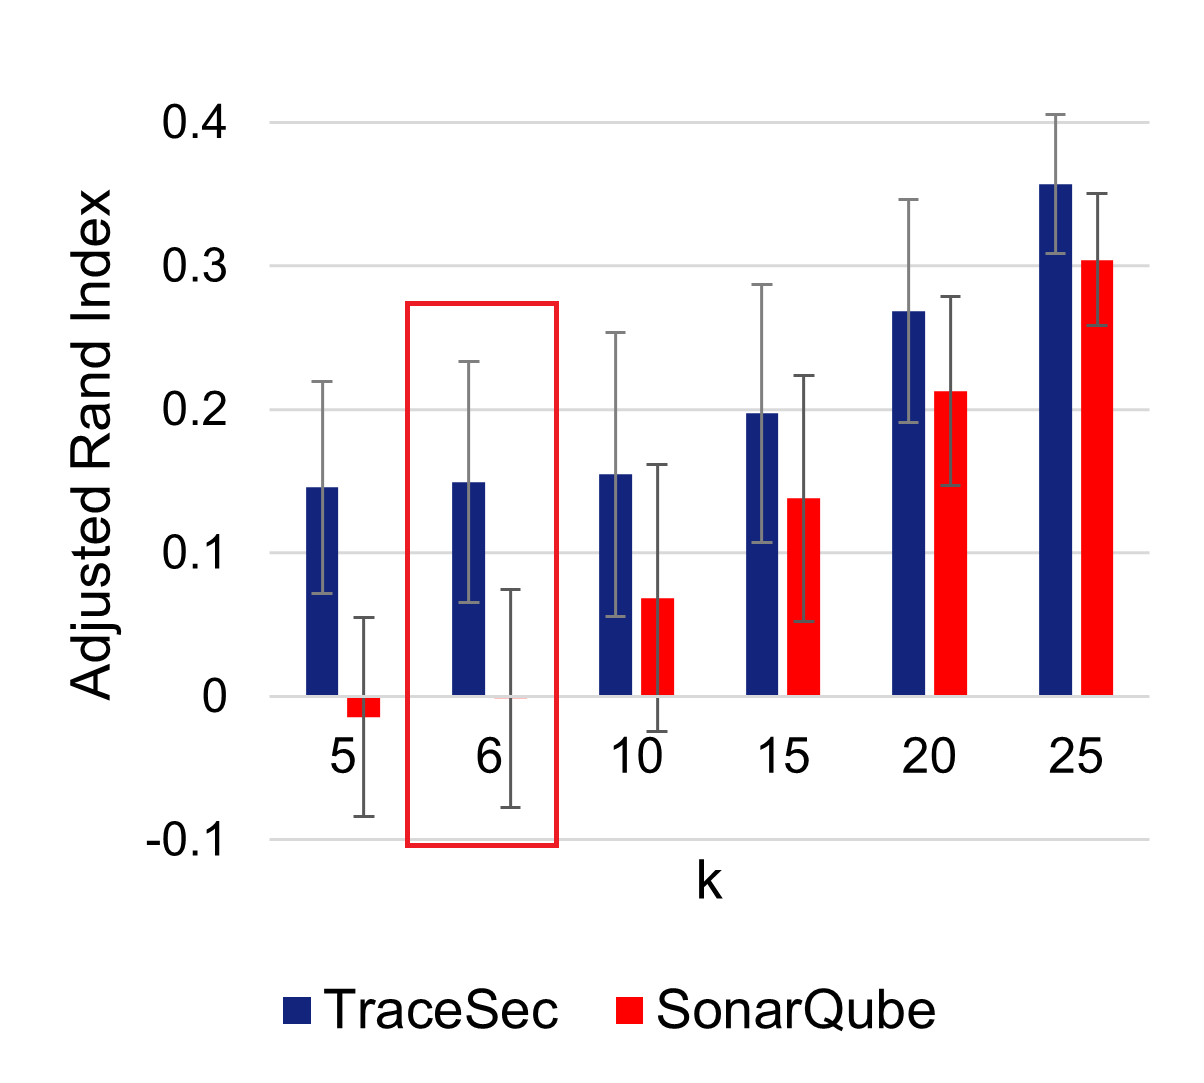
\includegraphics[width=.9\linewidth]{figures/topKiTrust}
		\caption{iTrust}
		\label{topKiTrust}
		\end{center}%
	\end{subfigure}%
	\begin{subfigure}{.5\textwidth}
		\begin{center}
		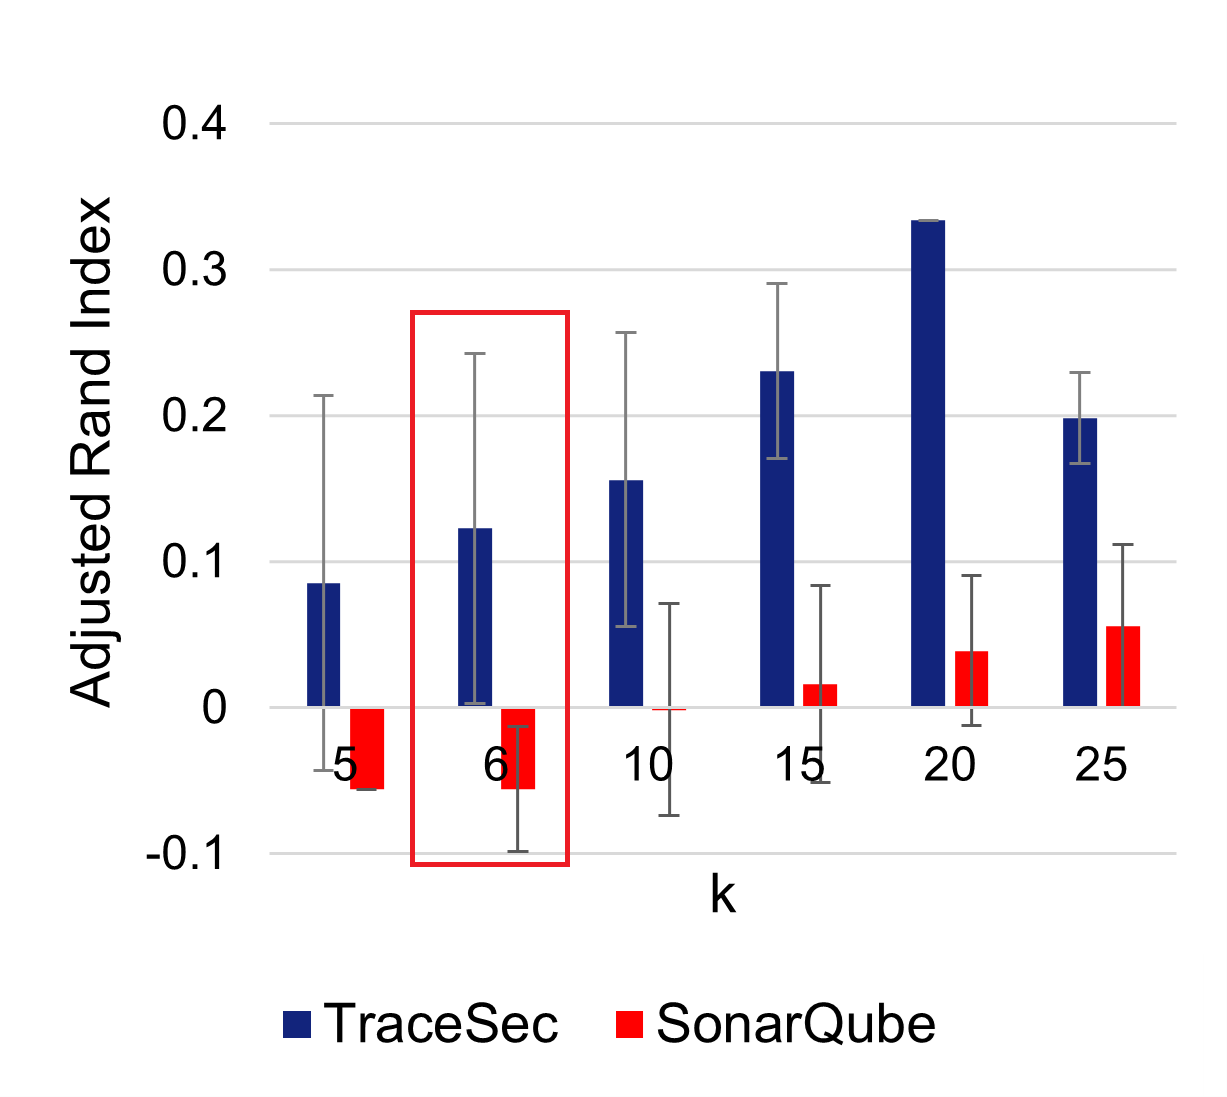
\includegraphics[width=.9\linewidth]{figures/topKcwa}%
		\caption{CWA}
		\label{topKCWA}
		\end{center}
	\end{subfigure}
	\caption{Adjusted Rand Index (ARI) for Partition of Top k Findings Compared to Manual Prioritization}
	\label{topK}
	\end{center}
\end{figure}

Thus, a more coarse grained comparison of the rankings based on clusters seems more appropriate.
In practice, developers are mainly interested in the most important issues to fix. To compare the two prioritizations in this regard, we checked %what percentage
the similarity
of the top k most important issues according to our manual prioritization %are also in
with
the top k most important issues according to the SonarQube rule priorities and \appr.
\autoref{topK} shows the Adjusted Rand Index~(ARI)\,\cite{Hubert1985,Santos2009} similarity of two-class partitions into top k and all other findings for k = 5 to 25.
The presented values are averages over 1,000 runs, where the issues with the same priority are randomly shuffled within that range.
These permutations make the evaluation robust against random effects of issues %sharing the same priority as others within the top-k group but
being cutoff from the top-k cluster due to ordering when there are more issues of the same priority than fit into the top-k.
The error-bars in \autoref{topK} indicate the respective standard deviation $\sigma$.
Here,  \appr\ clearly outperforms SonarQube.
The top 5, and for CWA also top 10, similarity of SonarQube is even lower than for a random partition.
%However, on CWA the similarity values are generally lower.
As can be seen in \autoref{fig:manual-ranks}, there are 6 issues for CWA that are labeled with a priority of 5 and higher, and 6 issues for iTrust that were manually labeled with a priority of 6 or higher.
Since all groups with lower priority labels become much larger, e.g., 12 additional issues for CWA with a priority of 4, we assume that these 6 issues are the most important issues for the two projects. %Accordingly, we choose k as 6 for the comparison.
%This choice of k also
Choosing k = 6
eliminates the possible randomness due to more issues being identically ranked than can be added to the top k group.
We highlight these values in \autoref{topK}.
The ARI similarity for the top 6 partition on iTrust is $0.15$ for \appr\ and $0.08$ for SonarQube.
On the CWA \appr\  achieves $0.12$ and SonarQube $-0.06$.
This matches the general pattern observed in \autoref{topK} and shows that \appr\ better reflects the priorities derived from project context as considered in the manual ranking.

As we do not have a real gold standard, the individual background of diverging ratings is relevant.
%Here we discuss some observations.
First, we observe that \appr{} does not distinguish issues within the test code from those in the actual system code.
In the manual rating, issues within the test code are treated more or less equally and generally rated to be of lower importance.
\appr{} reflects the dependencies of individual test cases to the main project and, thus, differentiates different cases.
Issues in test cases can cause falsely passed tests that do not test the intended behaviour.
We observed this in at least one case for iTrust.
Considering the importance of thorough testing in general and of security-critical functions specifically, to take this into account appears more plausible than the intuitive manual approach.

Issues with a low manual rating but medium priority in the flow analysis were  manually often considered false positives (of the static-analyzer tool) or irrelevant.
As stated above, our approach is not designed to detect false positives.
For that, the precision of the static analyzer itself would have to be increased, which is not the focus of this work.
Similarly, rules that are considered irrelevant, e.g., certain naming conventions, can be customized or deactivated.

In our dataset, we have a single outlier %issue #41
that is manually rated as rather important but has only low to medium importance concerning the flow analysis.
This particular issue resides in a field of a Java class that has only a few trace connections to the rest of the project.
Yet, it is accessible through the UI and, thus, exploitable.
Positively, this outlier still has in all three rankings a higher priority than other issues in the same class.
However, this shows potential for improvement, as fields are generally less connected with other artifacts than methods.
This needs to be addressed in parameter tuning in the configuration~file.%, which is examined in objective \ref{o2}.

%Considering the effort for the manual prioritization, already these results on the the small iTrust example with partially artificial re-engineerired artifacts and trace links with coarse granularity appear promising.


%iTrust is a small real world example.
%However, it is rather small and partially the artifacts and in particular the trace links are artificially re-engineered.
%The granularity of the traces is quite coarse grained.
%and size of sample (100) -> feasibility
%Discuss reliability of manual ranking vs. expected automated results / effort
%considering the manual effort for prioritization the result is close enough to help reduce work



\subsection{Adjustability}
To evaluate the adjustability to project-specific priorities~(\ref{o2}), we investigate the impact of weighting options as described in \autoref{edgeCap}.
While capacities of individual edge types can be adjusted through a configuration file using the presented DSL, as described in \autoref{DevArt}, the quality model is the most likely entry point for project-specific prioritization as this is where the stakeholder judgment is documented and applied.
The configuration file is only specified once by an expert and not edited during the usual development~process.

To evaluate the influence of these weighting instruments, we compare the results of the prioritization with different capacities for different quality aspects. %or edge types.

\subsubsection{Setup}
%We take again the 100 issues used for \ref{o1}.
%The priorities calculated in the effectiveness experiment serve as a reference.
We take again the 100 issues used for \ref{o1} and use the calculated priorities as a reference.
First, we investigate the impact of the priority values in the quality model by keeping the manual assignment of the priorities in the quality model %from the previous experiment
and multiplying these with different factors to get smaller and higher priorities.
In another run of the maximum flow analysis, we change the priorities in the quality model to assign a significantly higher priority to a single sub-tree of the quality model.
We compare the ordering analogously to the effectiveness evaluation \ref{o1}.

\subsubsection{Results}

\autoref{fig:weights} shows the correlations of the 100 issues prioritized using \appr{} with the prioritization from O1 for different capacities applied to a four-level ranking in the quality model.
The applied capacities are shown on the x-axis and are ordered increasingly.
The capacities used in O1 are 25-50-75-100.
Accordingly, this prioritization is identical with the one of O1, which corresponds with an R-value of 1.
Increasing the priorities further has no impact on the prioritization; with the capacities used in O1, the bottleneck of the flow network (known as \emph{minimum cut}\,\cite{1056816,ford_fulkerson_1956}) %(described as minimum cut in literature\,\cite{1056816,ford_fulkerson_1956})
is not in the quality model.
On the other hand, the lower capacities in the quality model lead to increasing differences in the prioritizations for iTrust, which is reflected by a lower R-value.
For the CWA, only capacities 1-2-3-4 lead to a slight difference with a correlation of .9999 instead of 1.
However, the correlation with the manual ranking improved slightly to .4711, indicating that the minimum cut has been moved into the quality model.
Unfortunately, as we only support natural numbers, reducing the weights further is not possible. Here, we suffer from the fact that the CWA only has a very abstract component diagram which allows few trace links that limit the capacity that can be propagated from the quality model towards the issues.

\begin{figure}
    \centering
    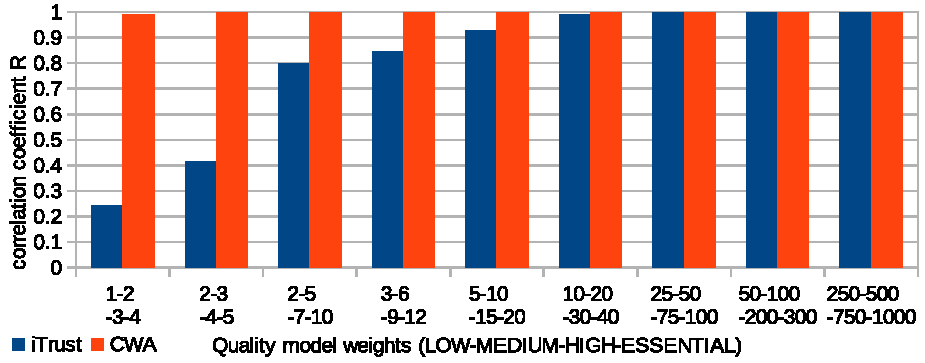
\includegraphics[width=.75\columnwidth]{figures/impact-qm-weights.pdf}
    \caption{Impact of the Priority Values in the Quality Model}
    %\caption{Impact of the Weight Values in the Quality Model on the Prioritization}
    \label{fig:weights}
\end{figure}

Altogether, choosing good capacities (representing the priorities in the quality model) is essential for a prioritization that reflects the importance of qualities.
If the capacity is chosen too low, the minimum cut through the network is located in the quality model and the other artifacts might have no impact on the prioritization.
If the capacities are chosen too high, the issues are only prioritized based on the other artifacts.
A suitable trade-off has to be found.
Whether the priorities in the quality model can influence the prioritization at all is discussed based on the second part of this evaluation~objective.

%\begin{figure}
%    \centering
%    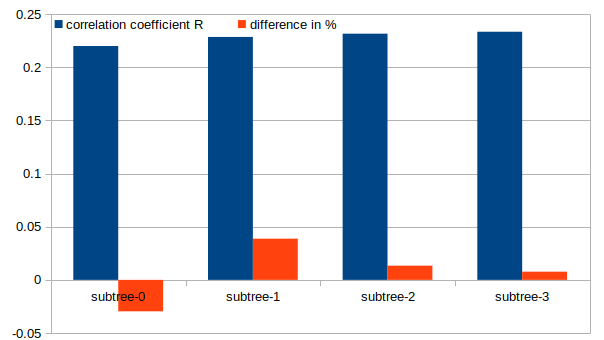
\includegraphics[width=\columnwidth]{figures/impact-qm-trees.png}
%    \caption{Impact of the prioritization of a single sub-tree of the quality model on the prioritization}
%    \label{fig:trees}
%\end{figure}

\autoref{tab:trees} shows the correlations of the prioritization from O1 with the prioritizations calculated when assigning high importance to only one of the sub-trees of iTrust's quality model and among each other.
With R-values close to 1 the
%single
prioritizations are very similar but still, the changes in the quality model show an effect on the prioritization.
As we already observed that the parts of the flow network representing the other artifacts played a central role in the prioritization, these results are not unexpected.
Still, it shows that already with a small and highly interconnected quality model users can influence the~prioritization.

For the CWA we got identical prioritizations (a correlation of~1) regardless of which tree was set to high importance.
As the highest ranked issue of the CWA only got a rating of 23, this is not surprising as in this experiment the lowest priority in the quality model reflects a capacity of 25.
As in the first part of this experiment, there are too few trace links between the quality model and the architecture.

\begin{table}
    \centering
    \caption{Correlation Matrix Showing the Impact of the Prioritization of a Single Sub-tree of iTrust's Quality Model}
    \label{tab:trees}
%    \footnotesize
    \begin{tabular}{r|rrrr}
        \toprule
         & tree 1 & tree 2 & tree 3 & tree 4  \\
         \midrule
        O1 & .9898 & .9919 & .9950 & .9897 \\
        tree 1 & & .9966 &	.9931 & .9997 \\
        tree 2 & & & .9965 &	.9969 \\
        tree 3 & & & & .9934 \\
        \bottomrule
    \end{tabular}
\end{table}


Overall, the influence of the quality model on prioritization is lower than expected.
The exemplary quality models are rather small and highly interconnected as they only contain essential security-related aspects.
Especially the CWA shows that a sufficient amount of trace links from the quality model to the other artifacts is necessary to allow adjustability.
We expect more influence for not reverse-engineered models with more project context.

\subsection{Robustness}

	Creating trace links is expensive and error prone and in practice imperfect trace links are likely.
	Besides this, particularly design models such as UML models are often rather less used in practice\,\cite{Gorschek2014} and if present are probably not of the highest quality.
	Therefore, we are interested in how well TraceSEC performs in presence of imperfect trace links and planning artifacts (\ref{o4}).
	The overall question is whether lesser organized projects can still benefit from \appr{}.
	To understand the quality requirements on needed artifacts such as models and trace links, we are going to investigate how the accuracy of traceability links, i.e., connections within models and trace links between models and code, affect the importance rankings.

\subsubsection{Setup}
	To estimate the impact of imperfect traceability, we need to consider two types of trace links separately.
	First, internal links within artifacts (requirements \& design models), and second, external links between different artifacts (QM → requirements → design → code).
	The former indicates the quality of the artifacts produced, while the latter indicates how well trace links between different artifacts are created and maintained.
	Therefore, we considered these two types of trace links independently.



	To evaluate how robust TraceSEC is to imperfect trace links, we injected faults into the trace links by randomly deleting existing trace links or randomly creating additional trace links.
	Additions and deletions were performed independently, and we iteratively added and deleted between 0\% and 50\% of all trace links.
	After each change, we measured the quality of the prioritization in terms of correlation with the manual baseline.
	Since only detailed requirements and design models are available for iTrust, we performed this experiment only on this case study.



\subsubsection{Results}
%
	In  \autoref{tab:robustness} we show how much the correlation with the manual base line changed for the addition of false positives (fp) and deletions leading to false negatives (fn).
	When looking at the outcomes, missing external trace links severely impact the prioritization. However, false positives do not seem to be a  problem (it is often better to have a wrong trace link instead of no trace link).
	Therefore, external trace links must not be precise and internal trace links can make up for not accurate external trace links.
	On their own, internal trace links have only a low impact.
	Since the used models of iTrust were reverse engineered from the code and therefore only few information is added, this could be an explanation for this observed low impact but therefore high robustness.
	However, there is still a slight negative impact.

\begin{figure}

	\begin{subfigure}{\textwidth}
		\footnotesize
		\setlength{\tabcolsep}{2pt}
		\centering
		\begin{tabularx}{\textwidth}{>{\bfseries}r|XXXXXXXXXXXXXXXX}
			fp\textbackslash fn &	\textbf{0.0\%} &	\textbf{0.1\%} &	\textbf{0.2\%} &	\textbf{0.5\%} &	\textbf{1.0\%} &	\textbf{2.0\%} &	\textbf{5.0\%} &	\textbf{10.0\%} &	\textbf{15.0\%} &	\textbf{20.0\%} &	\textbf{25.0\%} &	\textbf{30.0\%} &	\textbf{35.0\%} &	\textbf{40.0\%} &	\textbf{45.0\%} &	\textbf{50.0\%} \\
			\hline
			0.0\%   &	0.00\% &	\rcolor{0.00} &	\rcolor{0.00} & \rcolor{0.00} & \rcolor{-0.35} &	\rcolor{-0.36} & \rcolor{-1.49} & \rcolor{-4.21} & \rcolor{-6.43} & \rcolor{-6.43} & \rcolor{-6.53} & \rcolor{-7.36} & \rcolor{-7.70} & \rcolor{-8.59} & \rcolor{-9.94} & \rcolor{-12.09} \\
			0.1\%   &	\rcolor{1.29} & \rcolor{1.23} & \rcolor{1.23} & \rcolor{0.99} & \rcolor{0.73} & \rcolor{0.41} & \rcolor{-0.72} & \rcolor{-2.02} & \rcolor{-2.28} & \rcolor{-2.48} & \rcolor{-3.65} & \rcolor{-2.81} & \rcolor{-4.21} & \rcolor{-3.32} & \rcolor{-3.09} & \rcolor{-5.35} \\
			0.2\%   &	\rcolor{2.06} & \rcolor{2.01} & \rcolor{2.04} & \rcolor{2.02} & \rcolor{2.01} & \rcolor{2.39} & \rcolor{0.28} & \rcolor{-1.55} & \rcolor{-1.84} & \rcolor{-1.71} & \rcolor{-2.01} & \rcolor{-1.65} & \rcolor{-3.01} & \rcolor{-2.84} & \rcolor{-3.22} & \rcolor{-2.76} \\
			0.5\%   &	\rcolor{2.25} & \rcolor{2.17} & \rcolor{2.17} & \rcolor{2.17} & \rcolor{2.17} & \rcolor{2.17} & \rcolor{1.73} & \rcolor{0.24} & \rcolor{-1.03} & \rcolor{-0.73} & \rcolor{-1.86} & \rcolor{-2.88} & \rcolor{-2.93} & \rcolor{-3.29} & \rcolor{-4.67} & \rcolor{-4.93} \\
			1.0\%   &	\rcolor{2.25} & \rcolor{2.17} & \rcolor{2.17} & \rcolor{2.17} & \rcolor{2.17} & \rcolor{2.25} & \rcolor{1.59} & \rcolor{0.92} & \rcolor{0.72} & \rcolor{0.22} & \rcolor{0.28} & \rcolor{0.08} & \rcolor{-1.36} & \rcolor{-1.45} & \rcolor{-1.56} & \rcolor{-1.17} \\
			2.0\%   &	\rcolor{2.25} & \rcolor{2.17} & \rcolor{2.16} & \rcolor{2.16} & \rcolor{2.16} & \rcolor{1.63} & \rcolor{1.58} & \rcolor{1.65} & \rcolor{0.60} & \rcolor{-1.61} & \rcolor{-1.59} & \rcolor{-0.88} & \rcolor{-0.77} & \rcolor{-0.91} & \rcolor{-0.81} & \rcolor{-0.80} \\
			5.0\%   &	\rcolor{2.43} & \rcolor{2.35} & \rcolor{2.35} & \rcolor{2.35} & \rcolor{2.35} & \rcolor{2.35} & \rcolor{2.25} & \rcolor{1.99} & \rcolor{0.50} & \rcolor{0.55} & \rcolor{0.18} & \rcolor{-0.37} & \rcolor{0.01} & \rcolor{-0.64} & \rcolor{-0.59} & \rcolor{-0.62} \\
			10.0\%  &	\rcolor{2.42} & \rcolor{2.33} & \rcolor{2.33} & \rcolor{2.33} & \rcolor{2.33} & \rcolor{2.18} & \rcolor{2.21} & \rcolor{2.60} & \rcolor{2.32} & \rcolor{2.01} & \rcolor{2.15} & \rcolor{1.57} & \rcolor{1.33} & \rcolor{1.17} & \rcolor{1.14} & \rcolor{1.13} \\
			15.0\%  &	\rcolor{2.42} & \rcolor{2.33} & \rcolor{2.33} & \rcolor{2.33} & \rcolor{2.33} & \rcolor{2.33} & \rcolor{2.33} & \rcolor{1.68} & \rcolor{1.24} & \rcolor{1.23} & \rcolor{1.10} & \rcolor{1.03} & \rcolor{1.03} & \rcolor{0.91} & \rcolor{0.91} & \rcolor{0.92} \\
			20.0\%  &	\rcolor{2.42} & \rcolor{2.33} & \rcolor{2.33} & \rcolor{2.33} & \rcolor{2.33} & \rcolor{2.33} & \rcolor{2.33} & \rcolor{1.97} & \rcolor{1.97} & \rcolor{1.97} & \rcolor{1.97} & \rcolor{2.11} & \rcolor{1.79} & \rcolor{1.54} & \rcolor{1.54} & \rcolor{1.54} \\
			25.0\%  &	\rcolor{2.42} & \rcolor{2.33} & \rcolor{2.33} & \rcolor{2.33} & \rcolor{2.33} & \rcolor{2.33} & \rcolor{2.17} & \rcolor{2.17} & \rcolor{2.42} & \rcolor{1.81} & \rcolor{1.81} & \rcolor{1.90} & \rcolor{1.90} & \rcolor{1.95} & \rcolor{1.95} & \rcolor{1.95} \\
			30.0\%  &	\rcolor{2.42} & \rcolor{2.33} & \rcolor{2.33} & \rcolor{2.33} & \rcolor{2.33} & \rcolor{2.33} & \rcolor{2.33} & \rcolor{2.30} & \rcolor{2.30} & \rcolor{2.18} & \rcolor{2.30} & \rcolor{2.44} & \rcolor{2.19} & \rcolor{2.17} & \rcolor{2.17} & \rcolor{2.17} \\
			35.0\%  &	\rcolor{2.42} & \rcolor{2.33} & \rcolor{2.33} & \rcolor{2.33} & \rcolor{2.33} & \rcolor{2.33} & \rcolor{2.33} & \rcolor{2.33} & \rcolor{2.07} & \rcolor{1.97} & \rcolor{1.97} & \rcolor{2.07} & \rcolor{2.07} & \rcolor{2.07} & \rcolor{2.07} & \rcolor{2.07} \\
			40.0\%  &	\rcolor{2.42} & \rcolor{2.33} & \rcolor{2.33} & \rcolor{2.33} & \rcolor{2.33} & \rcolor{2.33} & \rcolor{2.33} & \rcolor{2.30} & \rcolor{2.30} & \rcolor{2.18} & \rcolor{2.18} & \rcolor{2.42} & \rcolor{2.42} & \rcolor{2.41} & \rcolor{2.41} & \rcolor{2.41} \\
			45.0\%  &	\rcolor{2.42} & \rcolor{2.33} & \rcolor{2.33} & \rcolor{2.33} & \rcolor{2.33} & \rcolor{2.33} & \rcolor{2.33} & \rcolor{2.33} & \rcolor{2.33} & \rcolor{2.21} & \rcolor{2.21} & \rcolor{2.33} & \rcolor{2.33} & \rcolor{2.33} & \rcolor{2.33} & \rcolor{2.33} \\
			50.0\%  &	\rcolor{2.42} & \rcolor{2.33} & \rcolor{2.33} & \rcolor{2.33} & \rcolor{2.33} & \rcolor{2.33} & \rcolor{2.33} & \rcolor{2.33} & \rcolor{2.33} & \rcolor{2.21} & \rcolor{1.92} & \rcolor{1.92} & \rcolor{1.92} & \rcolor{1.73} & \rcolor{1.73} & \rcolor{1.73} \\
		\end{tabularx}

		\caption{Changes for external trace links between different artifacts.}
	\end{subfigure}

	\begin{subfigure}{\textwidth}
		\footnotesize
		\setlength{\tabcolsep}{2pt}
		\centering
		\begin{tabularx}{\textwidth}{>{\bfseries}r|XXXXXXXXXXXXXXXX}
			fp\textbackslash fn &	\textbf{0.0\%} &	\textbf{0.1\%} &	\textbf{0.2\%} &	\textbf{0.5\%} &	\textbf{1.0\%} &	\textbf{2.0\%} &	\textbf{5.0\%} &	\textbf{10.0\%} &	\textbf{15.0\%} &	\textbf{20.0\%} &	\textbf{25.0\%} &	\textbf{30.0\%} &	\textbf{35.0\%} &	\textbf{40.0\%} &	\textbf{45.0\%} &	\textbf{50.0\%} \\
			\hline
			0.0\% & 0.00\% & \rcolor{0.00} & \rcolor{0.00} & \rcolor{0.00} & \rcolor{0.00} & \rcolor{0.00} & \rcolor{0.02} & \rcolor{0.06} & \rcolor{0.06} & \rcolor{0.02} & \rcolor{0.03} & \rcolor{0.03} & \rcolor{0.00} & \rcolor{0.02} & \rcolor{0.07} & \rcolor{0.09} \\
			0.1\% & \rcolor{-0.01} & \rcolor{-0.01} & \rcolor{-0.01} & \rcolor{-0.01} & \rcolor{-0.01} & \rcolor{-0.01} & \rcolor{-0.01} & \rcolor{0.00} & \rcolor{-0.05} & \rcolor{-0.04} & \rcolor{-0.08} & \rcolor{-0.08} & \rcolor{-0.07} & \rcolor{-0.01} & \rcolor{0.04} & \rcolor{0.03} \\
			0.2\% & \rcolor{0.00} & \rcolor{0.00} & \rcolor{0.00} & \rcolor{0.02} & \rcolor{0.01} & \rcolor{0.01} & \rcolor{-0.03} & \rcolor{-0.04} & \rcolor{-0.02} & \rcolor{-0.03} & \rcolor{-0.03} & \rcolor{-0.03} & \rcolor{-0.03} & \rcolor{-0.06} & \rcolor{-0.06} & \rcolor{-0.06} \\
			0.5\% & \rcolor{0.00} & \rcolor{0.00} & \rcolor{-0.01} & \rcolor{-0.01} & \rcolor{-0.01} & \rcolor{-0.01} & \rcolor{-0.01} & \rcolor{0.00} & \rcolor{0.03} & \rcolor{0.05} & \rcolor{0.05} & \rcolor{0.05} & \rcolor{0.02} & \rcolor{-0.01} & \rcolor{-0.01} & \rcolor{-0.01} \\
			1.0\% & \rcolor{-0.01} & \rcolor{-0.01} & \rcolor{-0.01} & \rcolor{-0.01} & \rcolor{-0.01} & \rcolor{-0.01} & \rcolor{-0.01} & \rcolor{-0.02} & \rcolor{0.02} & \rcolor{0.02} & \rcolor{0.01} & \rcolor{0.01} & \rcolor{0.01} & \rcolor{0.01} & \rcolor{0.01} & \rcolor{0.01} \\
			2.0\% & \rcolor{-0.02} & \rcolor{-0.02} & \rcolor{-0.01} & \rcolor{-0.01} & \rcolor{-0.01} & \rcolor{-0.01} & \rcolor{-0.01} & \rcolor{-0.02} & \rcolor{-0.01} & \rcolor{-0.01} & \rcolor{0.03} & \rcolor{0.03} & \rcolor{0.03} & \rcolor{0.03} & \rcolor{0.03} & \rcolor{0.02} \\
			5.0\% & \rcolor{-0.02} & \rcolor{-0.02} & \rcolor{-0.02} & \rcolor{-0.02} & \rcolor{-0.02} & \rcolor{-0.01} & \rcolor{-0.01} & \rcolor{-0.02} & \rcolor{0.06} & \rcolor{0.06} & \rcolor{0.06} & \rcolor{0.06} & \rcolor{0.05} & \rcolor{0.05} & \rcolor{0.05} & \rcolor{0.05} \\
			10.0\% & \rcolor{-0.06} & \rcolor{-0.06} & \rcolor{-0.06} & \rcolor{-0.06} & \rcolor{-0.06} & \rcolor{-0.06} & \rcolor{-0.06} & \rcolor{-0.07} & \rcolor{-0.07} & \rcolor{-0.07} & \rcolor{-0.07} & \rcolor{-0.07} & \rcolor{-0.06} & \rcolor{-0.06} & \rcolor{-0.06} & \rcolor{-0.06} \\
			15.0\% & \rcolor{-0.06} & \rcolor{-0.06} & \rcolor{-0.06} & \rcolor{-0.06} & \rcolor{-0.06} & \rcolor{-0.06} & \rcolor{-0.06} & \rcolor{-0.06} & \rcolor{-0.07} & \rcolor{-0.07} & \rcolor{-0.06} & \rcolor{-0.03} & \rcolor{0.18} & \rcolor{0.18} & \rcolor{0.18} & \rcolor{0.18} \\
			20.0\% & \rcolor{-0.06} & \rcolor{-0.06} & \rcolor{-0.06} & \rcolor{-0.06} & \rcolor{-0.06} & \rcolor{-0.06} & \rcolor{-0.06} & \rcolor{-0.06} & \rcolor{-0.07} & \rcolor{-0.07} & \rcolor{-0.07} & \rcolor{-0.07} & \rcolor{-0.04} & \rcolor{-0.04} & \rcolor{-0.04} & \rcolor{-0.04} \\
			25.0\% & \rcolor{-0.06} & \rcolor{-0.06} & \rcolor{-0.06} & \rcolor{-0.06} & \rcolor{-0.06} & \rcolor{-0.06} & \rcolor{-0.06} & \rcolor{-0.10} & \rcolor{-0.10} & \rcolor{-0.10} & \rcolor{-0.11} & \rcolor{-0.11} & \rcolor{-0.14} & \rcolor{-0.14} & \rcolor{-0.09} & \rcolor{-0.09} \\
			30.0\% & \rcolor{-0.06} & \rcolor{-0.06} & \rcolor{-0.06} & \rcolor{-0.06} & \rcolor{-0.06} & \rcolor{-0.06} & \rcolor{-0.06} & \rcolor{-0.06} & \rcolor{-0.05} & \rcolor{-0.05} & \rcolor{-0.05} & \rcolor{-0.05} & \rcolor{-0.05} & \rcolor{-0.05} & \rcolor{-0.05} & \rcolor{-0.05} \\
			35.0\% & \rcolor{-0.06} & \rcolor{-0.06} & \rcolor{-0.06} & \rcolor{-0.06} & \rcolor{-0.06} & \rcolor{-0.06} & \rcolor{-0.06} & \rcolor{-0.06} & \rcolor{-0.06} & \rcolor{-0.06} & \rcolor{-0.06} & \rcolor{-0.06} & \rcolor{-0.06} & \rcolor{-0.06} & \rcolor{-0.06} & \rcolor{-0.06} \\
			40.0\% & \rcolor{-0.06} & \rcolor{-0.06} & \rcolor{-0.06} & \rcolor{-0.06} & \rcolor{-0.06} & \rcolor{-0.06} & \rcolor{-0.06} & \rcolor{-0.06} & \rcolor{-0.06} & \rcolor{-0.06} & \rcolor{-0.06} & \rcolor{-0.06} & \rcolor{-0.06} & \rcolor{-0.06} & \rcolor{-0.06} & \rcolor{-0.06} \\
			45.0\% & \rcolor{-0.06} & \rcolor{-0.06} & \rcolor{-0.06} & \rcolor{-0.06} & \rcolor{-0.06} & \rcolor{-0.06} & \rcolor{-0.06} & \rcolor{-0.06} & \rcolor{-0.06} & \rcolor{-0.06} & \rcolor{-0.06} & \rcolor{-0.06} & \rcolor{-0.06} & \rcolor{-0.06} & \rcolor{-0.06} & \rcolor{-0.06} \\
			50.0\% & \rcolor{-0.06} & \rcolor{-0.06} & \rcolor{-0.06} & \rcolor{-0.06} & \rcolor{-0.06} & \rcolor{-0.06} & \rcolor{-0.06} & \rcolor{-0.06} & \rcolor{-0.07} & \rcolor{-0.07} & \rcolor{-0.07} & \rcolor{-0.07} & \rcolor{-0.07} & \rcolor{-0.07} & \rcolor{-0.07} & \rcolor{-0.07} \\
		\end{tabularx}
		\caption{Changes for internal trace links within requirements and design models.}
	\end{subfigure}

	\small
	\setlength{\tabcolsep}{2pt}
	\begin{tabular}{|c|c|c|c|c|c|c|c|c|c|c|c|c|}
		\cellcolor{Red} < -10\% &
		\cellcolor{Red!75} < -8\% &
		\cellcolor{BurntOrange!75} < -6\% &
		\cellcolor{YellowOrange!75} < -4\% &
		\cellcolor{Goldenrod!85} < -2\% &
		\cellcolor{Yellow!85} < -1\% &
		\cellcolor{Yellow!40} -1\% < \& < 1\% &
		\cellcolor{ForestGreen!17} > 1\% &
		\cellcolor{ForestGreen!33} > 2\% &
		\cellcolor{ForestGreen!50} > 4\% &
		\cellcolor{ForestGreen!67} > 6\% &
		\cellcolor{OliveGreen!70} > 8\% &
		\cellcolor{OliveGreen!100} > 10\%\\
	\end{tabular}

	\caption{Average change in correlation with the manual baseline after adding (fp) or deleting (fn) trace links.}
	\label{tab:robustness}
\end{figure}

\begin{figure}
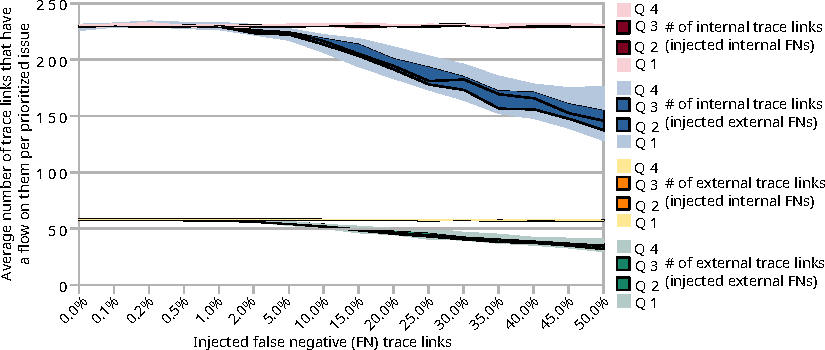
\includegraphics[width=.7\columnwidth]{figures/fns-edges.pdf}
\caption{Number of internal and external trace links used for prioritization dependent on the number of false negative trace links}
\label{fig:fnsEdges}
\end{figure}

\edit{
	To better understand the results, we measured for the cases in which we only injected false negatives (FNs), i.e., deleting external or internal trace links how many of the edges in the flow network corresponding to them carry a flow when prioritizing an issue and how much flow this is per edge.
	As visible in \autoref{fig:fnsEdges}, the number of as well internal as external trace links that have a flow on them decreases with the number of deleted external trace links (FNs).
	Thereby, the number of internal trace links decreases stronger than the number of external trace links.
	If internal trace links are deleted, the numbers stay consistent.
	This fits to the results shown in \autoref{tab:robustness}, in which we also do not see a change for deleted internal trace links.
	Since as well the number of external trace links as internal trace links over which a flow is propagated decreases with increasing FNs, this implies that combinations of previously unused internal trace links cannot compensate missing external trace links to a notable extend.
	Instead, with deleted external trace links entire sub-graphs become uncreachable.
	When measuring the average flow across each trace link, we observed the same behavior as the number of trace links, implying also that the utilization of the used trace links, i.e., propagating additional flow over previously not saturated trace links, does not increase.
}


\begin{figure}
	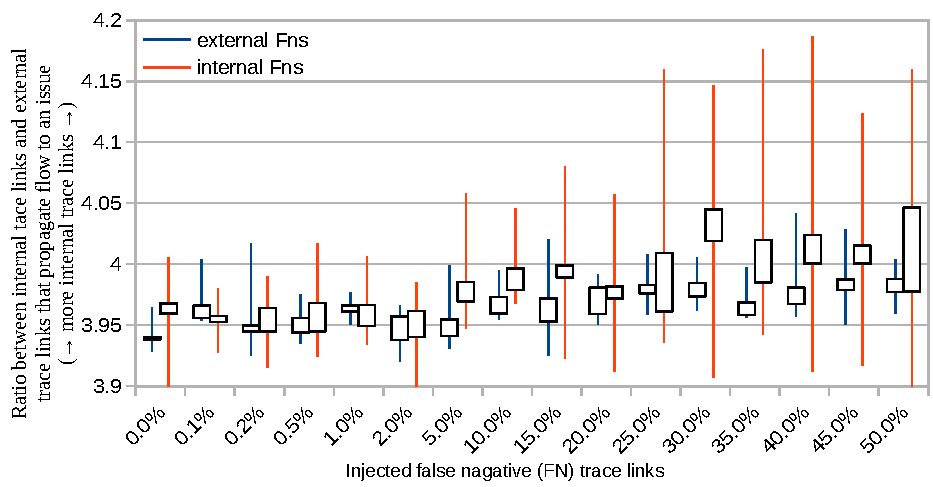
\includegraphics[width=.6\columnwidth]{figures/ratio-internal-to-external-tracelinks.pdf}
	\caption{Number of internal trace links to external trace links dependent on the number of false negative trace links}
	\label{fig:intVsExt}
\end{figure}

\edit{
	When comparing the usage of external and internal trace links in the prioritization, meaning over which of them flow is propagated, we notice that the higher the number of false negative trace links gets, the more internal trace links are involved in the prioritization of an issue (see \autoref{fig:intVsExt}).
	While this trend can be observed to some extent for both, false negative internal trace links and external trace links, it is more pronounced for deleted external trace links.
	This indicates that internal trace links, e.g., design models or derived from code, play an essential role in distributing importance allowing for external trace links not immediately pointing to concrete issue locations, and allow the prioritization to also function to some extent for missing external trace links.
}

Overall, this experiment indicates that even low quality design models and imperfect trace links are sufficient for gaining benefit from TraceSEC.
Considering alternatives such as the SonarQube rule priorities for prioritizing issues, even in the worst case in which 50\% of all trace links have been deleted (a 12.09\% lower correlation coefficient), the prioritization of TraceSec still correlates stronger with the manual base line than the prioritization based on rule priorities (a correlation coefficient of .4041 for TraceSEC, while, according to \autoref{tab:correlations}, SonarQube rule priorities resulted only in .3023).
Therefore, we can conclude that it is likely that even lesser organized projects can benefit from TraceSEC.
\edit{Our deeper investigation of how internal and external trace links behave in this experiment suggests that it may be more beneficial to optimize external trace links than internal trace links.
	However, since the two go hand in hand, artifacts containing internal trace links, such as requirements or design models, could be a means of optimizing external trace links between them.}

\subsection{Performance}
%
	Although often not explicitly measured, the continuous manual prioritization of issues adds significant overhead to the development of secure software systems.
	When only prioritizing issues and not interweaving this task with other development activities, the time we needed for prioritizing the issues of our baseline gives an indication of the involved overhead.
	Including discussions, the prioritization of 100 issues took us 120 minutes.
	Although, a single developer familiar with the project will be faster, significant overhead is still added.
	To this end, the automated prioritization of \appr{} aims at providing faster issue prioritization.
	To assess the benefit of \appr{}~(\ref{o3}), we have to consider two cost factors.
	First, unlike the manual prioritization \appr{} has an overhead for setting up the tooling.
	The second factor is the actual time needed for prioritization.




	\textit{1) Setup:}
	As discussed above, setting up \appr{} comes usually with relatively low cost since it works out of the box for most kinds of models.
	Custom models can be added to \appr{} by writing a few lines of configuration files.
	However, fine-tuning parameters, if needed, can be a significant effort but must not be invested upfront but we expect some continuous effort.
	Unfortunately, we have no practical experiences on this effort yet.
	For our own experiments, we needed less than 15 minutes to set up \appr{}, which included writing the needed configurations.


	\textit{2) Execution:}
	Wile the setup adds a static overhead, the actual execution of \appr{} takes time each time it is executed.
	Also, the time needed depends on the size of the flow network to create and analyze, i.e., the size of the project for which issues should be prioritized.
	Excluding the flow network construction, prioritizing 100 issues of iTrust (~70k LLOC) takes 23.9 seconds on average with TraceSEC.
	Since, the literature has extensively discussed the scalability of solving the max-flow problem and developed efficient algorithms\,\cite{ford_fulkerson_1956,dinic1970algorithm}, we expect no issues for larger projects.
To this end, for \ref{o3}, it remains to evaluate the scalability of the flow network~construction to determine the the performance gain of \appr{} compared to the manual prioritization.

\subsubsection{Setup}
%
To evaluate the scalability of constructing  flow networks, we measure the construction time for input data representing different-sized software projects. While plenty of real-world open-source Java projects exist that could be used, usually, requirements, design models, and trace links among them are not publicly available. For this reason, we randomly generated quality models, requirements models, component diagrams, and program models representing software projects of different sizes.

We have to ensure at model construction that the relation of nodes and references among these nodes corresponds with these of real-world projects.
Thus, we start with generating program models whose node and reference distributions correspond to those of 20 program models created in other works from real-world projects of different sizes (ranging from 1,197 to 201,541 logical lines of code)\,\cite{peldszus2016continuous,Peldszus2022}.
Afterward, we clustered the types contained in the program model for creating a UML component diagram as well as trace links.
Thereby, each cluster of types is linked to a component in the requirements diagram and the relations among the types are aggregated to inter component connections.
For each of these components, we generated two to four requirements and arranged these in the requirements model according to the relations observed in iTrust's requirements model.
Finally, we randomly generated a quality model whose size correlates with the number of requirements and randomly added trace links to these.
This way, we achieve input data whose relation among nodes and edges and also the relation among the sizes of the different models is realistic.
Furthermore, as we know the sizes of program models for software projects of different sizes from literature\,\cite{peldszus2016continuous}, we can state to which project size in terms of lines of code the generated models relate.

Using this generation approach, we generated random input data of different sizes with realistic distributions of nodes, relations, and trace links for which we measured the time required to construct the flow network.
We generated input data corresponding to projects between sizes of
%200,000 and 4,000,000
200k and 4x10$^6$
logical lines of code (LLOC) in steps of 100k %100,000
LLOC. For every size, we generated 10 different samples and report the average values.

\subsubsection{Results}
%
\autoref{fig:scaleability} shows the execution times of the flow network construction for input data representing software projects of different sizes.
As expected, the measured time increases with the input data size.
For medium-sized projects (below one million lines of code), we stay below two minutes that allows issue prioritization during development in an IDE.
For larger projects with up to three million lines of code, creation is possible on a consumer notebook (Intel i7-1165G7, 32GB RAM) in below one~hour.

\begin{figure}
    \centering
    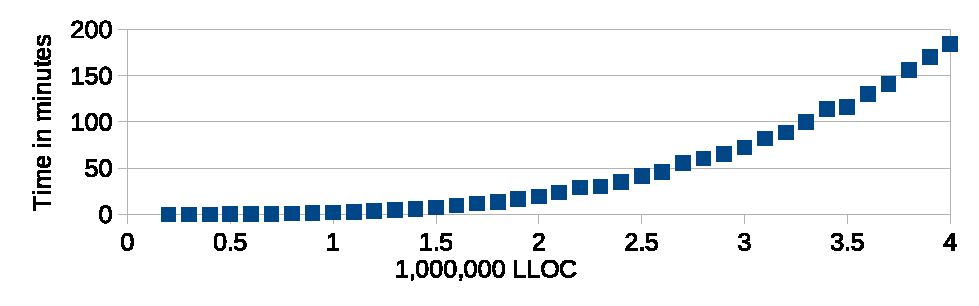
\includegraphics[width=.65\columnwidth]{figures/tracesec-scalability.eps}
    \caption{Scalability of the Flow Network Construction}
    \label{fig:scaleability}
\end{figure}

The scalability of the current implementation suffers from exponential time requirements when adding new elements to the base models (quality model, requirements, etc.) because the trace model has to be built anew with each change.
In future work, the prioritization could be calculated based on model deltas on a continuous integration server, which could then present the prioritized issues.

	Overall, it is likely that even a single execution of \appr{} saves enough time compared to manual prioritization to make up for the setup overhead.
	Assuming that \appr{} is executed with every nightly build, this allows for continuous prioritization of detected issues while saving significant time usually spent for manual prioritization.
	Even if some additional time is spent to optimize the configuration of \appr{}, e.g., monthly or quarterly taking two hours---the time we needed for one manual prioritization of 100 issues---to check whether there are observations such as the one described by us of noticing overly many edges due to accesses, this still saves significant effort.
